\documentclass[hidelinks]{article}

\usepackage[final,nonatbib]{nips_2016}

\usepackage[pdftex]{graphicx}		% including of figures, etc
\usepackage{float}					% alignment of tables/figures 
\usepackage[utf8]{inputenc} 		% allow utf-8 input
\usepackage[T1]{fontenc}    		% use 8-bit T1 fonts
\usepackage{hyperref}       		% hyperlinks
\usepackage{url}            		% simple URL typesetting
\usepackage{booktabs}       		% professional-quality tables
\usepackage{amsfonts}       		% blackboard math symbols
\usepackage{amsmath}				% math equation stuff
\usepackage[detect-none]{siunitx} 	% si units, range and stuff
\usepackage{nicefrac}       		% compact symbols for 1/2, etc.
\usepackage{microtype}      		% microtypography
\usepackage{subcaption}				% subfigures

% graphicx: Where should graphics be found?
\graphicspath{ {figures/} }

% Setup range symbol.
\sisetup{range-phrase = \text{--}}


% =============================================================================

\title{Deep Features to Track}

\author{
  Parker Lusk\thanks{Code available at \url{www.github.com/plusk01/deep-features}} \\
  Brigham Young University \\
  parker.lusk@byu.edu
  }

\begin{document}

\maketitle

% -----------------------------------------------------------------------------

\begin{abstract}
Almost all vision-based algorithms (deep learning and otherwise) rely on finding a set of lower dimensional features from a higher dimensional image space. In the visual tracking problem, salient features of the target(s) being tracked are selected using one of a variety of feature detector algorithms. Features are then corresponded across video frames and those measurements are passed to a filtering and data association stage. The bottleneck of most target trackers is the vision based frontend. The purpose of this work is to consider the computational efficiency and tracking accuracy of a convolutional network based approach.
\end{abstract}

\section{Introduction}

The impact of deep learning has spread to more than just the machine learning community. In particular, deep learning has vastly changed the way that high level image processing tasks such as image classification and image segmentation are carried out. An important way that deep neural network architectures are able to solve these algorithmically challenging problems is by the way that it handles multi-dimensional features in image space.

Researchers are currently working on further understanding how and why deep neural networks (DNNs) "learn" what they do when tasked with minimizing error. A large part of successful deep learning is prerequisite on proper choice of cost function. Similarly, the DNN "building blocks" chosen seem to affect the type of features selected by DNNs. It is interesting, however, that DNNs built for image processing tasks (see Section~\ref{sec:CNN}) seem to learn the same things at the lower levels of the architecture, largely agnostic to the depth of the architecture, the cost function, and the end task.

These lower level layers of image processing architectures seem to be learning filters for feature detection (see Section~\ref{sec:feature_detection}). The purpose of this report is to determine the usefulness of replacing traditional feature detectors with the the features extracted from a pre-trained deep neural network, specifically from \texttt{VGG} (see Section~\ref{sec:vgg}). This is known as transfer learning. It is of most interest to use these deep feature detectors in the application of visual multiple target tracking, explained below. This work considers the computational efficiency and the tracking accuracy of using a pre-trained feature detector over a traditional feature detector algorithm.

Work in this area has been emerging \cite{Yosinski2014, Zhang2015, Li2016}, but commonly is only for single target tracking. An approach that is similar to this approach is found in \cite{Hong2015}. This approach uses a saliency map of high-level, semantic features along with an SVM to track a single target. It is compared to the popular TLD tracker \cite{Kalal2010}. A major difference between this work and the work done by Hong \texttt{et al.} is where the features are extracted from.  Since \cite{Hong2015} takes features from the highest semantic layer, more processing must be done before features can be extracted. This also implies that the specific architecture of the neural network becomes important. In this paper, features are extracted from the second layer, minimizing computation and dependence on architecture layout.

% -----------------------------------------------------------------------------

\section{Visual Multiple Target Tracking}
Visual target tracking is an important component of many robotics applications. The need for vision-based tracking in many different settings has given rise to multiple solutions for this problem, each carrying their own assumptions. For example, a popular and well known feature tracker is the Lucas-Kanade Tracker, which uses optical flow to track featuere points across frames. This tracker constrains the camera to be on a static platform and assumes that the track(s) persists in the frame the entire duration of processing. This is a problem for robust tracking.

In the BYU MAGICC Lab, visual target tracking is an important subsystem of an integrated unmanned aerial system (UAS), or more colloquially, a drone. Not only is the platform moving, but it is necessary to track multiple dynamic targets that may come into and/or leave the field-of-view of the camera. The Recursive-RANSAC \cite{Niedfeldt2014, Defranco2015} algorithm was developed by the BYU MAGICC Lab to address these concerns.

Recursive-RANSAC is the core algorithm that can handle multiple target tracking in clutter, using a RANSAC approach to initialize tracks and a Kalman filter to update tracks and associate measurements according to a nearly constant acceleration (NCA) motion model. When applied to visual multiple target tracking (visual MTT), R-RANSAC is a powerful tool for generating and predicting the tracks of moving ground targets.

Currently, the vision processing frontend is the speed bottleneck of R-RANSAC-based visual MTT. In order to somewhat alleviate this, the incoming video streams is decimated by 3 -- meaning only 10 frames per second are used of the 30 fps footage. The job of the vision processing frontend is to generate measurements of moving objects to pass to R-RANSAC, which can then decide if a measurement is part of a current track, a new track, or simply clutter. A Good Features to Track detector is employed to find features, which are then matched to the next frame using a Lucas-Kanade Optical Flow pyramid. Feature points are then corrected using a homography that registers images and helps account for egomotion caused by movemement of the UAS.

At every iteration the Good Features to Track (GFTT) detector is run to generate feature points. The purpose of this report is to consider the use of a pre-trained neural network for feature extraction instead of the GFTT detector and to compare computational efficiency and tracking accuracy.

% -----------------------------------------------------------------------------

\section{Feature Detectors}\label{sec:feature_detection}
Many computer vision based algorithms start with the detction and extraction of features from an input image. As a result, many flavours of feature detection have been developed, each with its own strengths and weaknesses. Feature detectors are most robust when the computational complexity is low and there is repeatability of finding the same features given the same input.

There are four common types of image features: \textit{edges}, \textit{corners}, \textit{blobs}, and \textit{ridges}. The Harris and the Shi-Tomasi corner detectors are two methods in wide use today and will be discussed below.

\subsection{Harris Corner Detector}
The Harris corner detector \cite{Harris1988} is an improvement to Moravec's corner detector \cite{Moravec1980}, which considered a window of the image and determined the average changes of image intensity that result from shifting the window by a small amount in prescribed directions. Harris and Stephens mathematically formalized Moravec's heuristic through the eigenvalues of the $2x2$ matrix of the windowed gradients of the image, given by

\begin{equation}
M =
\begin{bmatrix}
  w*I_x^2 & w*I_x I_y \\
  w*I_x I_y & w*I_y^2
\end{bmatrix},
\end{equation}

where $*$ denotes convolution, $w$ is the window (typically Gaussian), and $I_x$ and $I_y$ are the partial derivatives of the image $I$.

By diagonalizing $M$ using eigenvalue decomposition, Harris and Stephens gave meaning to the eigenspace of $M$ as illustrated in \cite[Figure~5]{Harris1988}. Their results show the following for a given pixel $(x_0, y_0)$ in the image $I(x, y)$:

\begin{enumerate}
  \item If $\lambda_1 \approx 0$ and $\lambda_2 \approx 0$ then this region is flat and has no corner.
  \item If $\lambda_1 \approx 0$ and $\lambda_2 \gg 0$ then this region has an edge.
  \item If $\lambda_1 \gg 0$ and $\lambda_2 \gg 0$ then this region has a corner.
\end{enumerate}

Noting that matrix diagonalization can be computationally expensive, Harris and Stephens define a measure of cornered-ness using the properties $tr(M) = \lambda_1 + \lambda_2$ and $det(M) = \lambda_1 \lambda_2$. Their corner/edge response function is defined as

\begin{equation}\label{eq:harris_corn_meas}
  R = det(M) - \kappa\ tr^2(M),
\end{equation}

where $\kappa$ is a tunable sensitivity parameter, empirically found to typically be in the range of \numrange{0.04}{0.15}.

\subsection{Good Features to Track}
Building off of the work of Harris, Stephens, and Moravec, six years after the Harris corner detector paper was published, Shi and Tomasi proposed a different measure of cornered-ness than equation~\ref{eq:harris_corn_meas}:

\begin{equation}
  min(\lambda_1, \lambda_2) > \lambda_{th}.
\end{equation}

If this inequality holds for some threshold $\lambda_{th}$, the current window is accepted. Note that the eigenvalues must be directly computed for this method. The Shi-Tomasi argument is that under certain assumptions, the corners are more stable for tracking.

% -----------------------------------------------------------------------------

\section{Convolutional Neural Networks}\label{sec:CNN}

\subsection{Background}
Convolutional Neural Networks (CNNs or ConvNets) are a particular class of deep learning algorithms that have recently proved to be very powerful in image processing tasks. ConvNets are a type of feed-forward deep artificial neural network that consists of layers that process visual information in a hierarchical manner. Each layer is composed of small computational units known as convolutions, which essentially take a weighted average of regions of the input using a small filter (or kernel), typically on the order of a $3x3$ matrix. The weights of these filters are "learned" during back-propagation at test-time. This matrix of weights, or filter, is slide across the entire input to create what is called a feature map: a differently filtered version of the input image. See Figure~\ref{fig:conv_layer} for an illustration of a convolutional layer.

\begin{figure}[H]
  \centering
  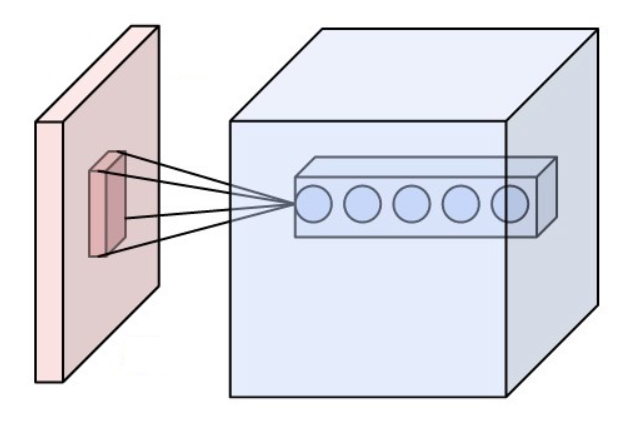
\includegraphics[scale=0.35]{conv_layer}
  \caption{Representation of a convolutional layer, showing an image (left) being scanned by a filter that has different weights at each depth of the output feature maps (right). Any given convolutional layer outputs a set of feature maps, defined by the depth of a layer. See \url{https://en.wikipedia.org/wiki/Convolutional_neural_network}}
  \label{fig:conv_layer}
\end{figure}

These convolutional layers are at the core of CNNs and is why they differ from vanilla deep neural networks (DNNs). A DNN is essentially a multilayer perceptron (MLP) with many hidden fully-connected layers. Because of the inherently spatial nature of images, convolutional layers do better than fully-connected layers as they preserve some level of spatial correlation of features. A typical CNN architecture is shown in Figure~\ref{fig:typical_cnn}.

Convolutional neural networks have been shown to do very well recently in supervised learning, often measured by the ability to classify the natural images from the ImageNet dataset. A flagship example of the power of CNNs is the AlexNet architecture\cite{Krizhevsky2012}, further improved on by the GoogLeNet \cite{Szegedy2014} and VGG \cite{Simonyan2015} architectures. The VGG architecture is shown in Figure~\ref{fig:vgg16}.

\begin{figure}[H]
  \centering
  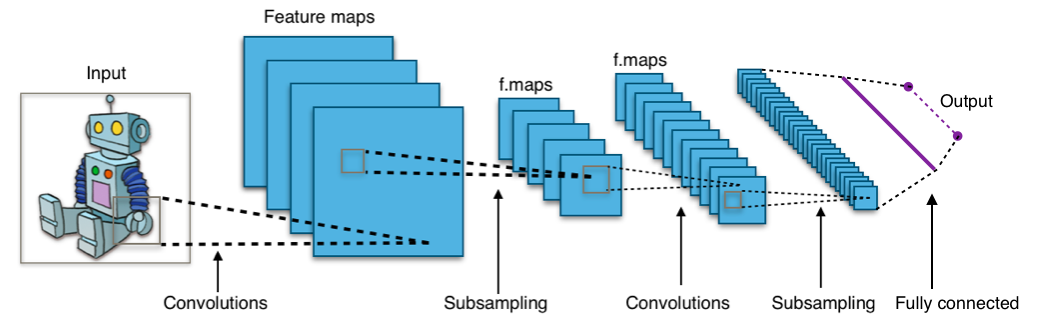
\includegraphics[scale=0.30]{typical_cnn}
  \caption{Typical CNN architecture, consisting mainly of convolutional layers.
    \newline See \url{https://en.wikipedia.org/wiki/Convolutional_neural_network}}
  \label{fig:typical_cnn}
\end{figure}

\subsection{Visualizing Feature Maps}
With all of the recent advances in deep neural networks in general and with convolutional neural networks in particular, it is becoming increasingly important to understand how they work. Our comprehension of how these models work and what these biologically-inspired neural nets are "thinking" has lagged behind our successes with them. This is especially true in the hidden layers in between the input and output layers.

Work has been progressing in this area, however, as researchers crack open the black box that is ConvNets. A popular method is to generate images that maximize the "activations" (the magnitude of the feature maps) in each layer \cite{Zeiler2014, Yosinski2015, Simonyan2014}. In \cite{Yosinski2015}, Yosinki \textit{et al.} develop a software tool that allows introspection of a convolutional neural network, as shown in Figure~\ref{fig:deepviz}. Use of this tool increases one's intuition of layers and the features that each layer in the hierarchy look for. It turns out that as an image advances in the ConvNet hierarchy, the amount of semantic information increases, i.e., beginning layers pick out task-independent features (edges, corners, etc) while layers toward the end of a CNN pick out more contextual information (book, face, dog, etc).

\begin{figure}[H]
  \centering
  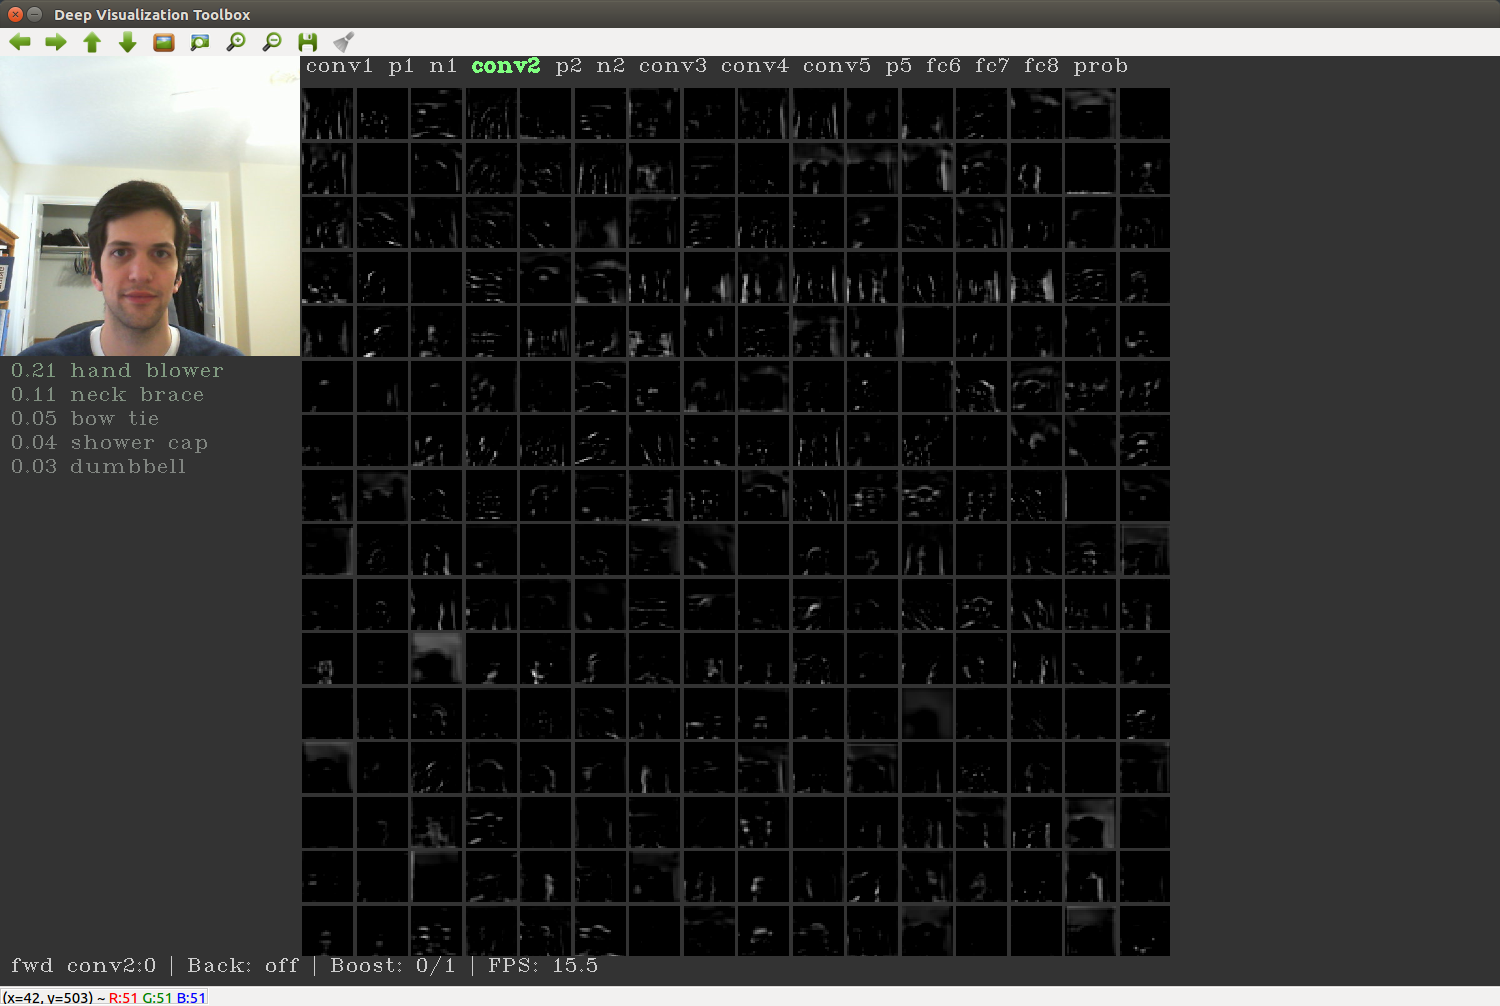
\includegraphics[scale=0.17]{deepviz}
  \caption{Yosinksi's Deep Visualization Toolbox \cite{Yosinski2015}, written in Caffe, running locally and connected to a camera. Note how the feature maps show where the \texttt{conv2} layer has found features from the camera feed of the author. Best if viewed electronically.}
  \label{fig:deepviz}
\end{figure}

\subsection{VGG Architecture}\label{sec:vgg}
In this paper, Oxford's pre-trained \texttt{VGG}, implemented in \texttt{Tensorflow} by Davi Frossard, was used for feature extraction. \texttt{VGG} expects input images to be $244x244$ and was trained on the whole of the ImageNet dataset. See Figure~\ref{fig:vgg16} for an illustration of each of the layers of VGG and \cite{Simonyan2015} for a discussion on the effectiveness of \texttt{VGG}.

\begin{figure}[H]
  \centering
  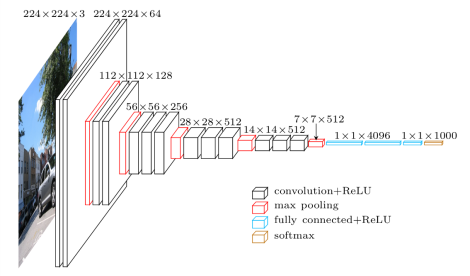
\includegraphics[scale=0.84]{vgg16}
  \caption{Architecture of VGG16 from Oxford's Visual Geometry Group \cite{Simonyan2015}. Taken from \newline \url{https://www.cs.toronto.edu/~frossard/post/vgg16/}.}
  \label{fig:vgg16}
\end{figure}


% -----------------------------------------------------------------------------

\section{Method}
In order to compare the efficiency and accuracy of a transfer learning approach, a basic visual tracking framework was built in Python 2.7 with OpenCV 2.4.13. Using data captured on Brigham Young University campus (see Appendix~\ref{app:campus}), the tracking framework was tested using the Good Features to Track feature detector, shown in Figure~\ref{fig:visual_mtt_gftt}.

\begin{figure}[H]
  \centering
  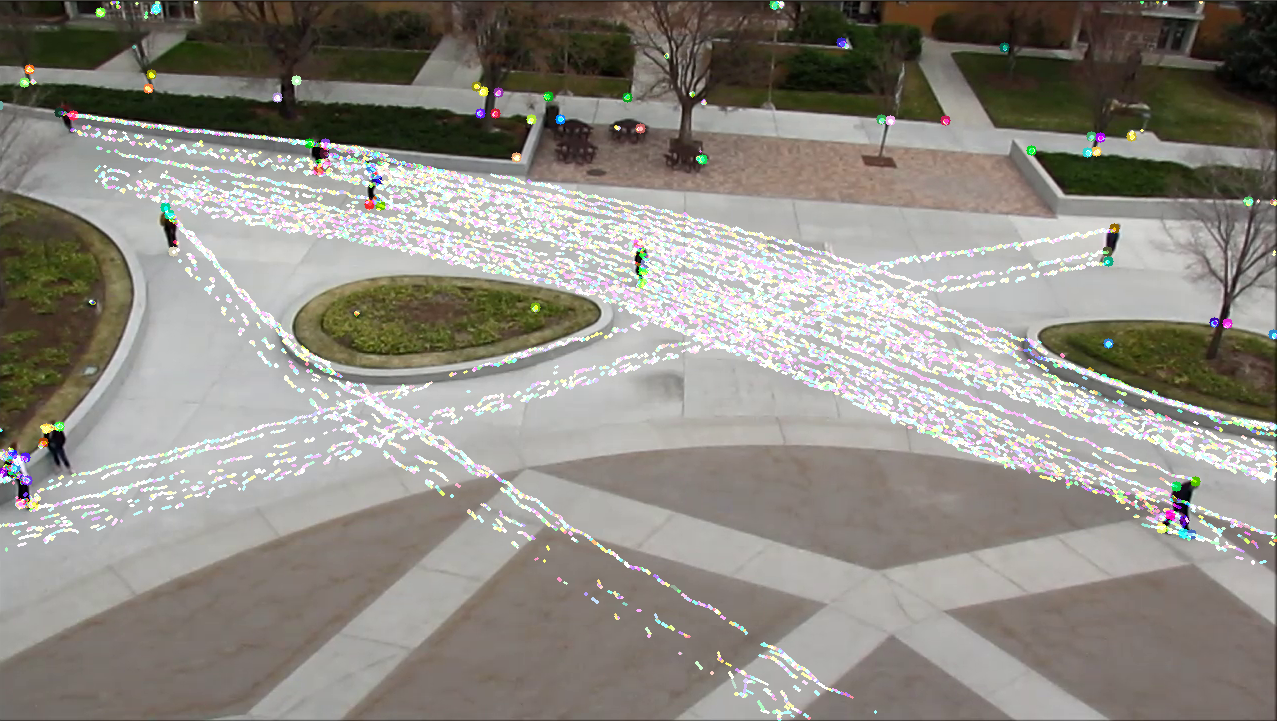
\includegraphics[scale=0.27]{visual_mtt_gftt}
  \caption{Visual multiple target tracking using Good Features to Track and LK Optical Flow.}
  \label{fig:visual_mtt_gftt}
\end{figure}

After finding features in the previous frame, the Lucas-Kanade Optical Flow tracker was used. LK Optical Flow takes features from an previous timestep and finds where they are at the current timestep, given the current frame. This allows for a computation of target motion in the image plane. Note in Figure~\ref{fig:visual_mtt_gftt} the nice smooth trajectories generated by the targets (erm...students) walking across the courtyard. Multiple trajectories are generated per target because the GFTT detector typically finds multiple features per person. The Python visual mtt framework ran at about 18 fps of the 29.97 fps from the footage.

Then, using Tensorflow and a pre-trained \texttt{VGG16} model, the GFTT detector was swapped out for the \texttt{conv1\_2} layer of \texttt{VGG16}. As the input footage was $1280x760$, it had to be scaled down and have black borders added to allow it to fit on \texttt{VGG}'s $224x224$ receptive field.

In order to decide which layer to use of \texttt{VGG}, the feature maps of the first four layers (\texttt{conv1\_1}, \texttt{conv1\_2}, \texttt{conv2\_1}, \texttt{conv2\_2}) were displayed and filters in each layer were hand-picked to test (See Appendix~\ref{app:fmap}). The aim in picking filters was to maximixe the intensity of features that represented targets. It was empirically found that the $45$th filter of \texttt{conv1\_2} was best suited for tracking multiple human targets from the given altitude, as shown in Figure~\ref{fig:fmap_orig}.

\begin{figure}[H]
  \centering
  \begin{subfigure}{0.49\textwidth}
    \centering
    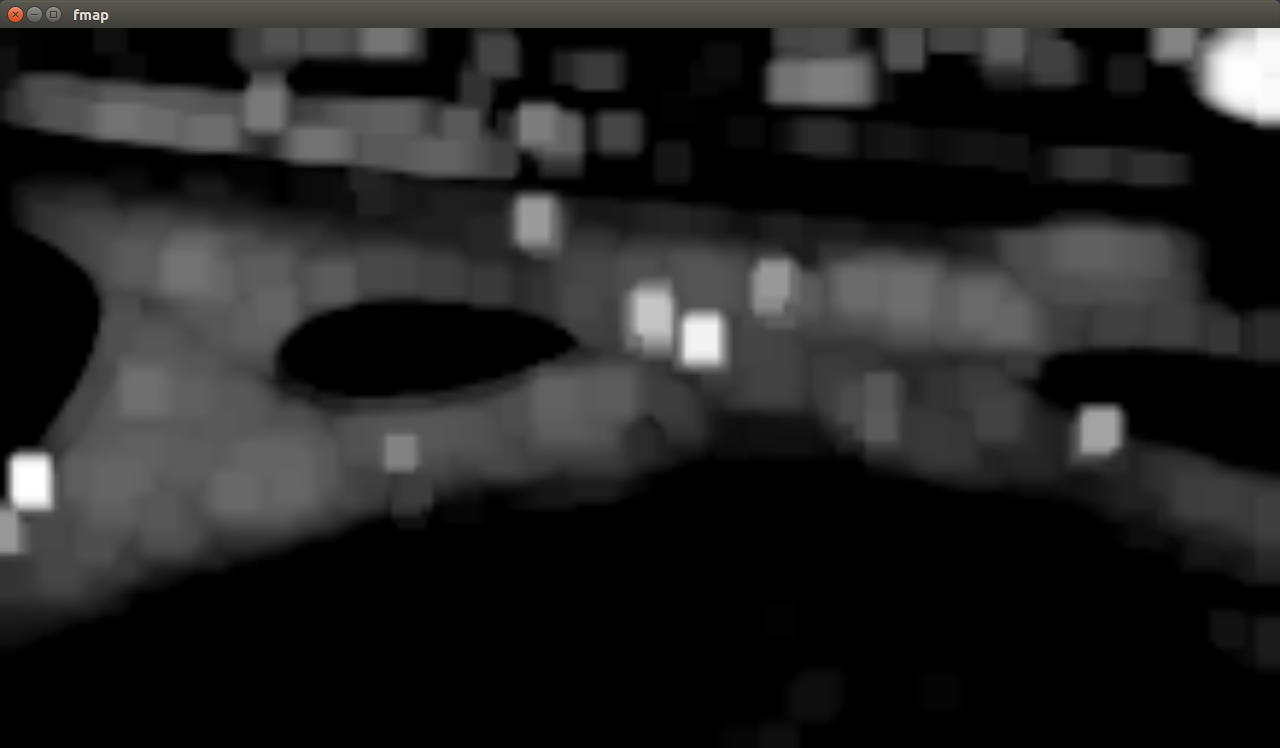
\includegraphics[width=\textwidth]{fmap}
    \caption{Original}
    \label{fig:fmap_orig}
  \end{subfigure}
  \begin{subfigure}{0.49\textwidth}
    \centering
    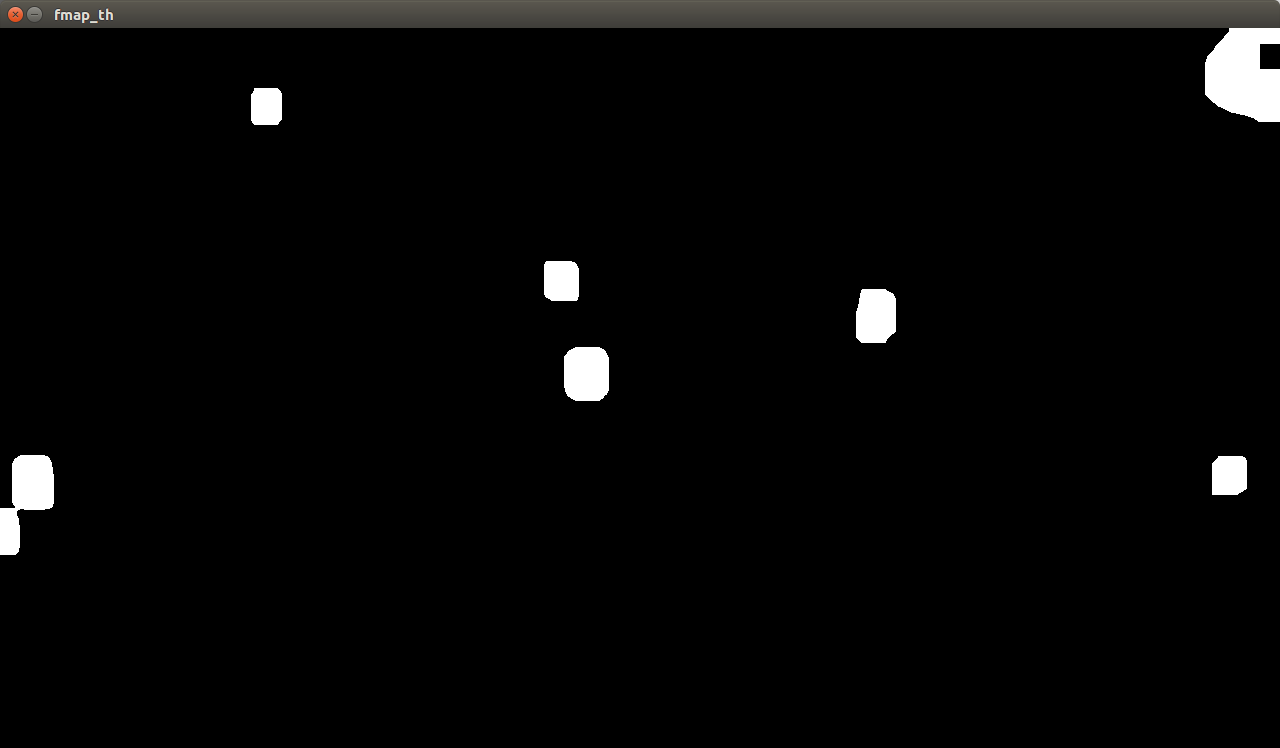
\includegraphics[width=\textwidth]{fmap_th}
    \caption{Thresholded}
    \label{fig:fmap_thresh}
  \end{subfigure}
  
  \caption{Feature map $45$ of \texttt{conv1\_2} at frame 100.}
  \label{fig:fmap}
\end{figure}

In order to reduce the number of features passed to LK Optical Flow, a simple kmeans algorithm was employed to find the 10 best blob centers from the thresholded image (Figure~\ref{fig:fmap_thresh}) of the feature map. The centroids of those blobs were then passed on to LK Optical Flow as had the GFTT features. The result of using deep features is shown in Figure~\ref{fig:deep_feature_track}. The trajectories are much less smooth than when using GFTT. Using deep features, processing ran at about 8 fps, much slower than with GFTT.

\begin{figure}[H]
  \centering
  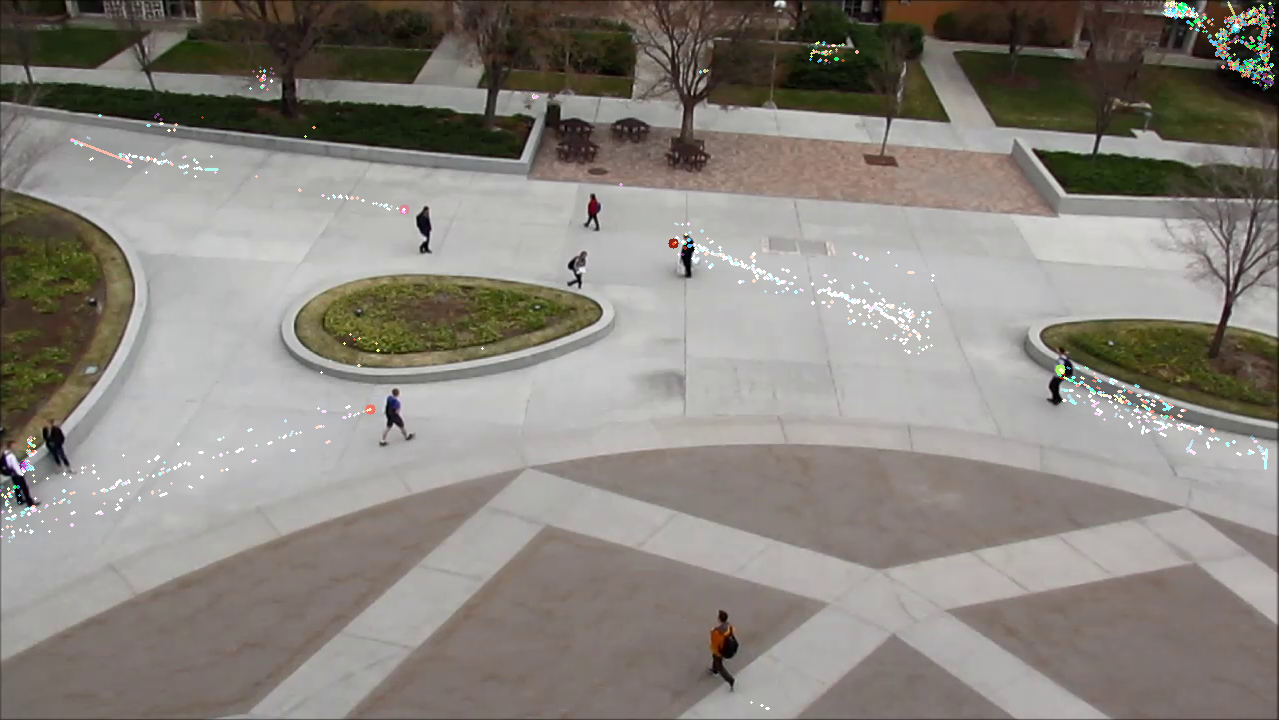
\includegraphics[scale=0.27]{deep_feature_track}
  \caption{Visual multiple target tracking using deep features and LK Optical Flow. Note that the feature output is less consistent, and there is an erroneous feature blob in the upper-righthand corner.}
  \label{fig:deep_feature_track}
\end{figure}

% -----------------------------------------------------------------------------

\section{Conclusion}
As can be surmised by Figures \ref{fig:visual_mtt_gftt} and \ref{fig:deep_feature_track} alone, the application of transfer learning to the visual multiple target tracking problem was not very successful. Not only was the Good Features to Track method more consistent across frames, but the trajectories created were smooth and it was much more computationally efficient.

While the framework and the deep features method may be tuned to give better feature results, it seems that it is a weaker solution as it is much more troublesome to tune and setup. 

A few closing thoughts:
\begin{itemize}
  
  \item It would be better to automatically iterate through filters and compare against output of GFTT on original frame to find the best filter to extract features from.
  
  \item This method assumes that the pre-trained weights were trained on images that contained the target.

  \item If nothing else, I have learned some things about formatting \LaTeX\ documents :)
  
\end{itemize}

\begin{thebibliography}{99}
\small

\bibitem{Niedfeldt2014} P. C. Niedfeldt, “Recursive-RANSAC: A Novel Algorithm for Tracking Multiple Targets in Clutter,” All Theses Diss., no. July, p. Paper 4195, 2014.

\bibitem{Defranco2015} P. C. Defranco, R. W. Beard, K. F. Warnick, and T. W. Mclain, “Detecting and Tracking Moving Objects from a Small Unmanned Air Vehicle,” no. March, 2015.

\bibitem{Shi1994} J. Shi and C. Tomasi, “Good Features to Track,” Pattern Recognit., no. June, 1994.

\bibitem{Harris1988} C. Harris and M. Stephens, “A Combined Corner and Edge Detector,” Procedings Alvey Vis. Conf. 1988, pp. 147–151, 1988.

\bibitem{Moravec1980} H. P. Moravec, “Obstacle avoidance and navigation in the real world by a seeing robot rover.,” tech. Rep. C., p. 175, 1980.

\bibitem{Hong2015} S. Hong, T. You, S. Kwak, and B. Han, “Online Tracking by Learning Discriminative Saliency Map with Convolutional Neural Network,” CoRR, vol. abs/1502.0, 2015.

\bibitem{Zhang2015} K. Zhang, Q. Liu, Y. Wu, and M.-H. Yang, “Robust Visual Tracking via Convolutional Networks,” arXiv, pp. 1–18, 2015.

\bibitem{Li2016} H. Li, Y. Li, and F. Porikli, “DeepTrack: Learning Discriminative Feature Representations Online for Robust Visual Tracking,” IEEE Trans. Image Process., vol. 25, no. 4, pp. 1834–1848, 2016.

\bibitem{Kalal2010} Z. Kalal, K. Mikolajczyk, and J. Matas, “Tracking-learning-detection,” IEEE Trans. Pattern Anal. Mach. Intell., vol. 6, no. 1, pp. 1409–1422, 2010.

\bibitem{Krizhevsky2012} A. Krizhevsky, I. Sutskever, and G. E. Hinton, “ImageNet Classification with Deep Convolutional Neural Networks,” Adv. Neural Inf. Process. Syst., pp. 1–9, 2012.

\bibitem{Szegedy2014} C. Szegedy, W. Liu, Y. Jia, P. Sermanet, S. Reed, D. Anguelov, D. Erhan, V. Vanhoucke, A. Rabinovich, C. Hill, and A. Arbor, “Going Deeper with Convolutions,” 2014.

\bibitem{Simonyan2015} K. Simonyan and A. Zisserman, “Very Deep Convolutional Networks for Large-Scale Image Recognition,” Int. Conf. Learn. Represent., pp. 1–14, 2015.

\bibitem{Yosinski2015} J. Yosinski, J. Clune, A. Nguyen, T. Fuchs, and H. Lipson, “Understanding Neural Networks Through Deep Visualization,” Int. Conf. Mach. Learn. - Deep Learn. Work. 2015, p. 12, 2015.

\bibitem{Yosinski2014} J. Yosinski, J. Clune, Y. Bengio, and H. Lipson, “How transferable are features in deep neural networks?,” Adv. Neural Inf. Process. Syst. 27 (Proceedings NIPS), vol. 27, pp. 1–9, 2014.

\bibitem{Zeiler2014} M. D. Zeiler and R. Fergus, “Visualizing and understanding convolutional networks,” Lect. Notes Comput. Sci. (including Subser. Lect. Notes Artif. Intell. Lect. Notes Bioinformatics), vol. 8689 LNCS, no. PART 1, pp. 818–833, 2014.

\bibitem{Simonyan2014} K. Simonyan, A. Vedaldi, and A. Zisserman, “Deep Inside Convolutional Networks: Visualising Image Classification Models and Saliency Maps,” Iclr, p. 1-, 2014.


\end{thebibliography}

% =============================================================================
\newpage
\appendix
\section{Selected Frames from Campus Video} \label{app:campus}
The following video was used to test multiple target tracking. It is $720x1280$ footage recorded at $29.97$ fps from the top of the Joseph Fielding Smith Building at BYU. These poor students don't know the amount of times they have been ran through a tracking algorithm \texttt{:/}

\begin{figure}[h]
  \centering
  \begin{subfigure}{0.49\textwidth}
    \centering
    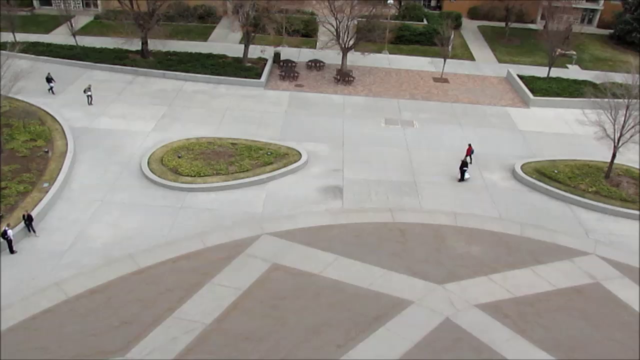
\includegraphics[width=\textwidth]{frame_0}
    \caption{Frame 0}
  \end{subfigure}
  \begin{subfigure}{0.49\textwidth}
    \centering
    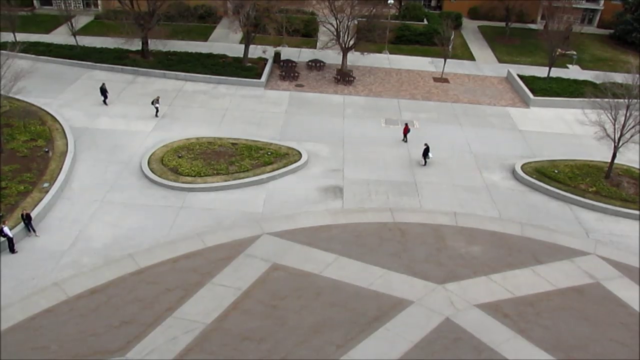
\includegraphics[width=\textwidth]{frame_100}
    \caption{Frame 100}
  \end{subfigure}
  \begin{subfigure}{0.49\textwidth}
    \centering
    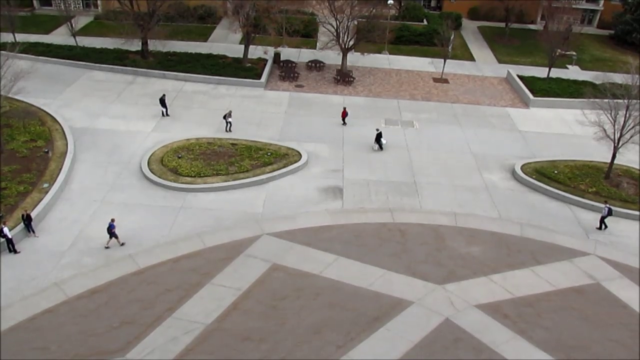
\includegraphics[width=\textwidth]{frame_200}
    \caption{Frame 200}
  \end{subfigure}
  \begin{subfigure}{0.49\textwidth}
    \centering
    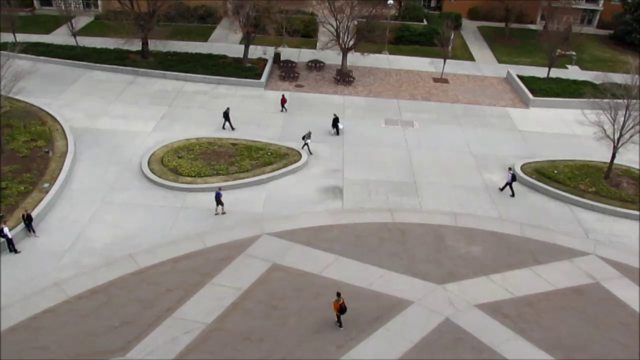
\includegraphics[width=\textwidth]{frame_300}
    \caption{Frame 300}
  \end{subfigure}
  
  \caption{Selected frames from the \texttt{campus.mp4} video.}
  \label{fig:campus_frames}
\end{figure}

% -----------------------------------------------------------------------------
\newpage
\section{Feature Map Visualization Images} \label{app:fmap}
Below, the activations (otherwise known as feature maps) of four layers of \texttt{VGG} are shown. Best if viewed electronically.

\begin{figure}[H]
  \centering
  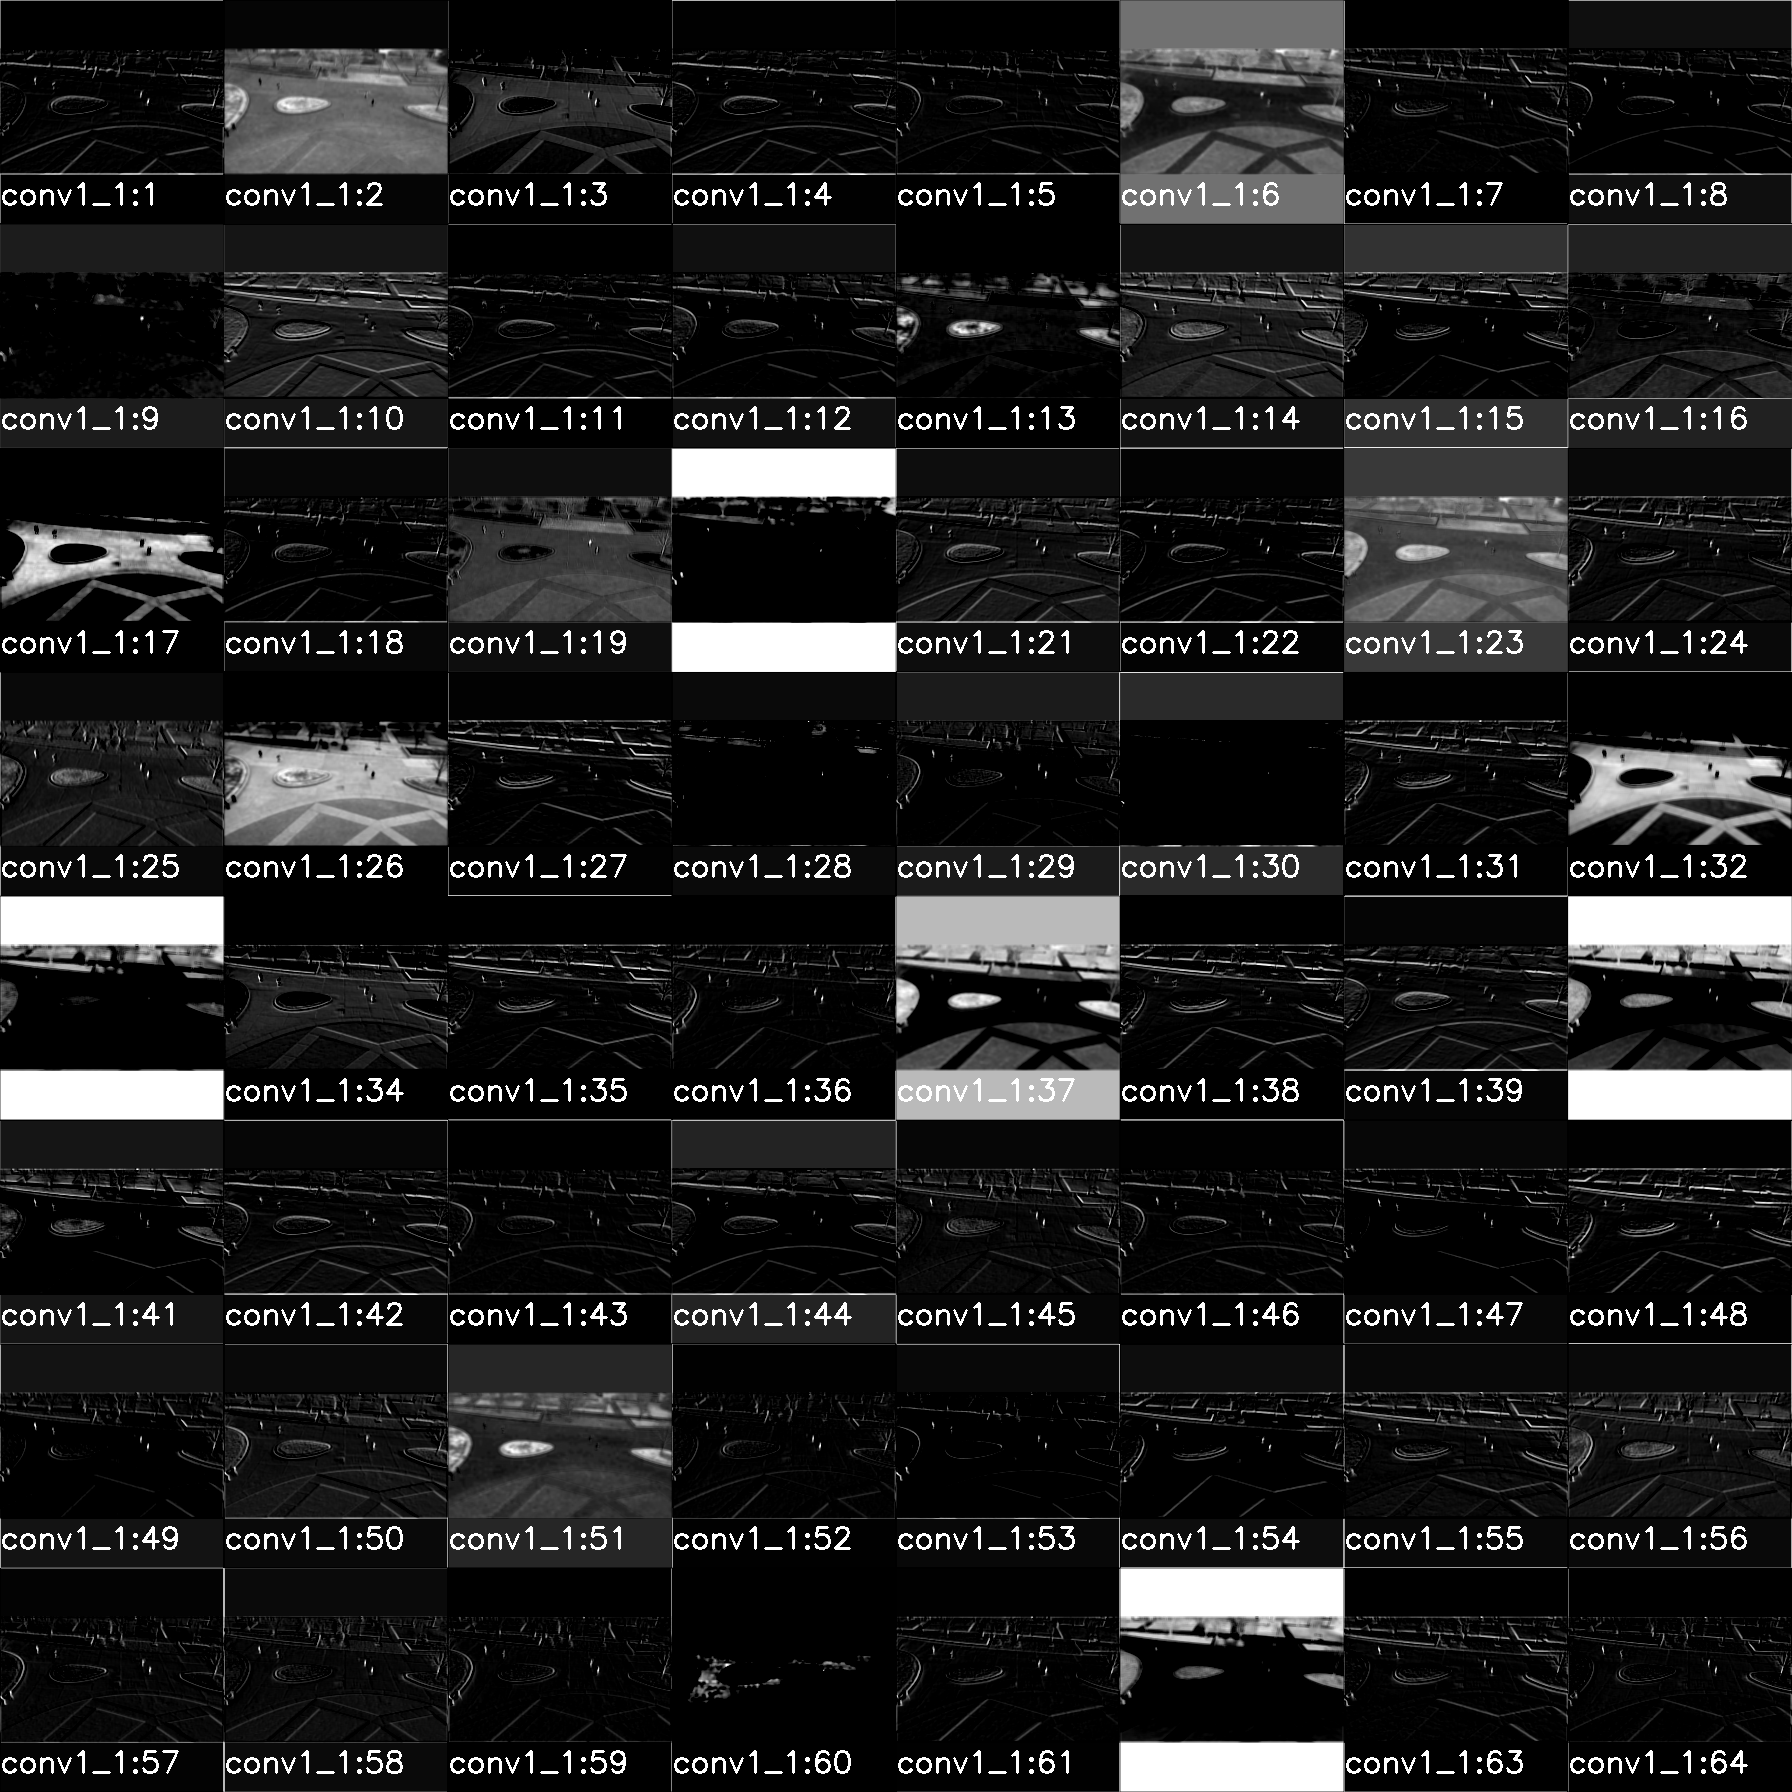
\includegraphics[scale=0.23]{acts_conv1_1}
  \caption{Feature maps of VGG16 layer \texttt{conv1\_1} at frame 100 of the \texttt{campus} video.}
  \label{fig:acts_conv1_1}
\end{figure}

\begin{figure}[H]
  \centering
  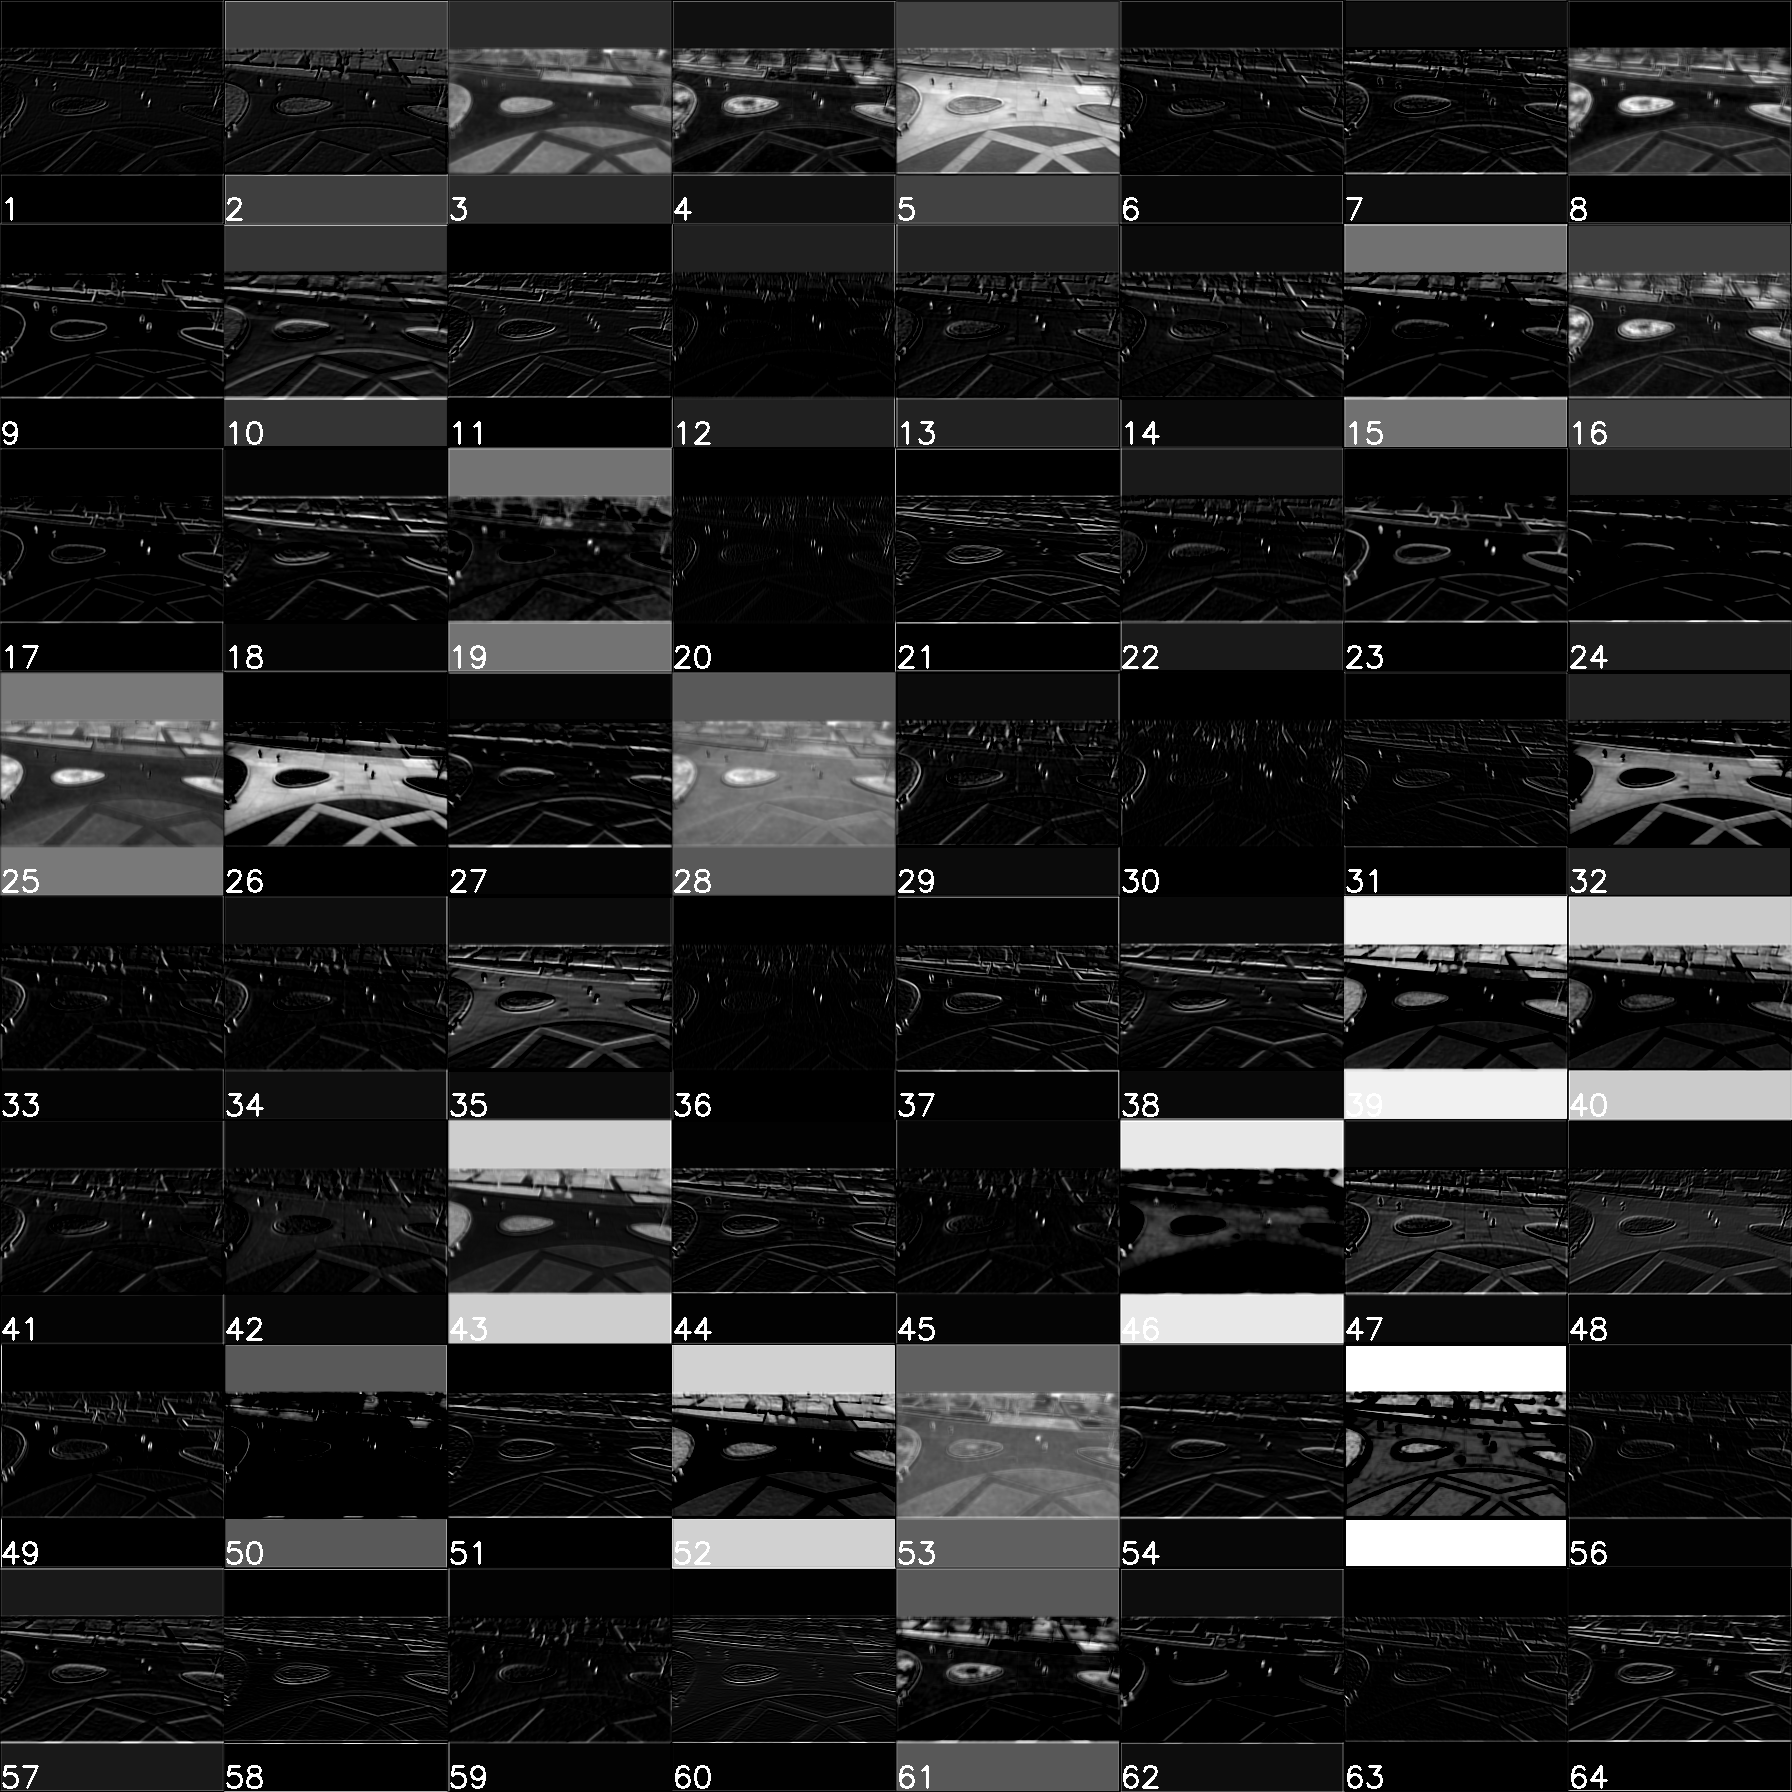
\includegraphics[scale=0.23]{acts_conv1_2}
  \caption{Feature maps of VGG16 layer \texttt{conv1\_2} at frame 100 of the \texttt{campus} video.}
  \label{fig:acts_conv1_2}
\end{figure}

\begin{figure}[H]
  \centering
  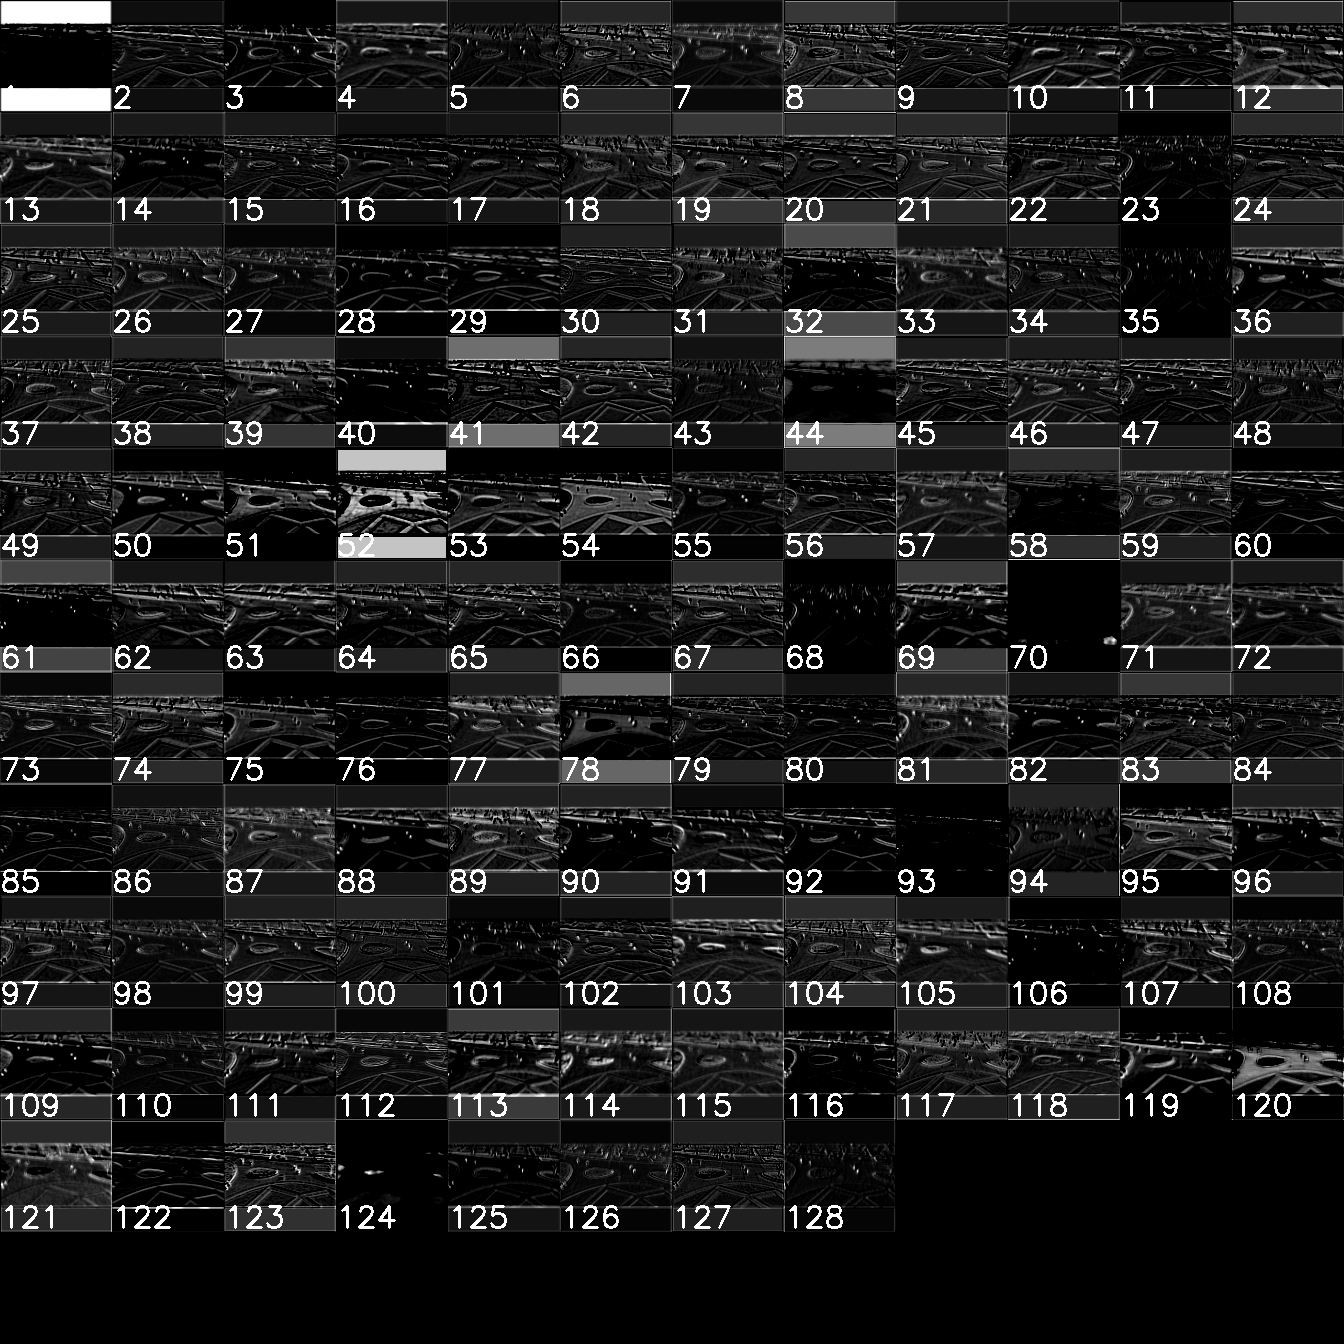
\includegraphics[scale=0.30]{acts_conv2_1}
  \caption{Feature maps of VGG16 layer \texttt{conv2\_1} at frame 100 of the \texttt{campus} video.}
  \label{fig:acts_conv2_1}
\end{figure}

\begin{figure}[H]
  \centering
  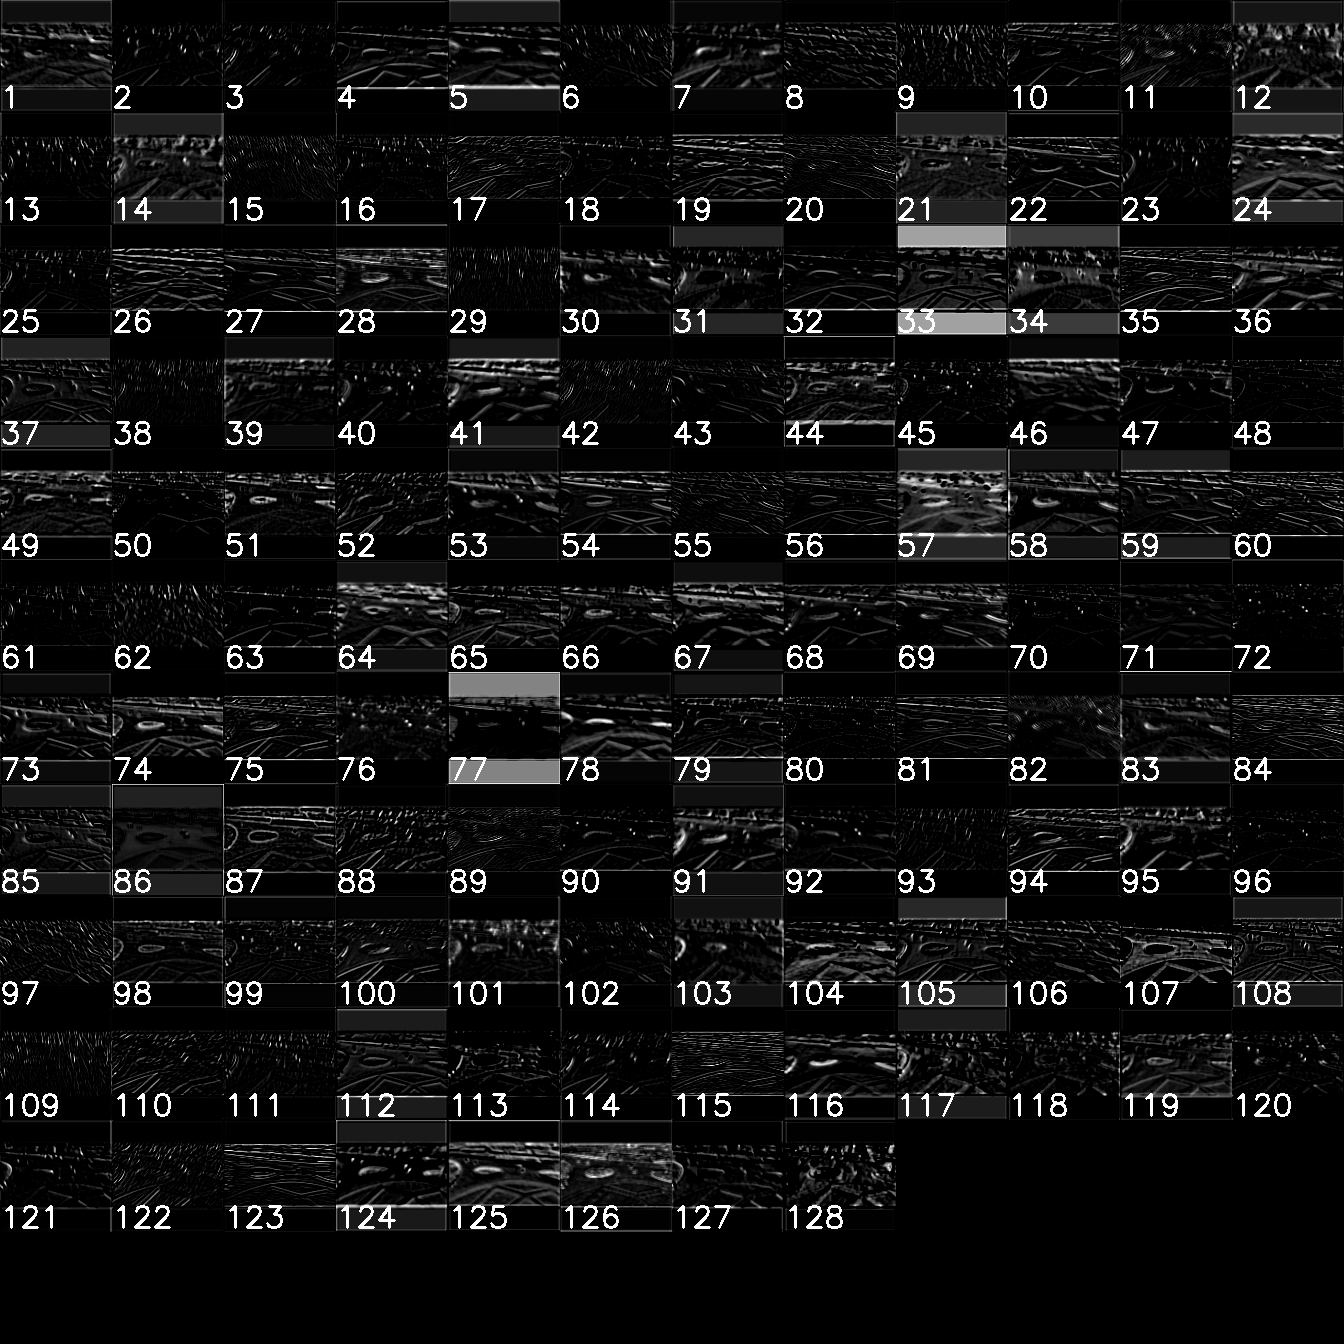
\includegraphics[scale=0.30]{acts_conv2_2}
  \caption{Feature maps of VGG16 layer \texttt{conv2\_2} at frame 100 of the \texttt{campus} video.}
  \label{fig:acts_conv2_2}
\end{figure}

\end{document}
